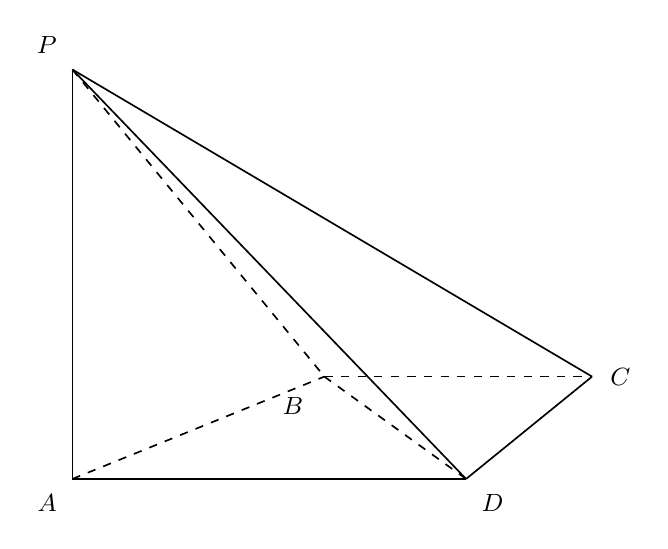
\begin{tikzpicture}[line width=.6pt, font=\small]
\coordinate (P) at (0,5.2);
\coordinate (A) at (0,0);
\coordinate (D) at (5,0);
\coordinate (C) at (6.6,1.3);
\coordinate (B) at (3.2,1.3);
% solid edges
\draw (P) -- (A);
\draw (A) -- (D);
\draw (D) -- (C);
\draw (P) -- (D);
\draw (P) -- (C);
% dashed hidden edges
\draw[dashed] (A) -- (B);
\draw[dashed] (B) -- (C);
\draw[dashed] (B) -- (D);
\draw[dashed] (P) -- (B);
\node[above left=2pt] at (P) {$P$};
\node[below left=2pt] at (A) {$A$};
\node[below right=2pt] at (D) {$D$};
\node[right=3pt] at (C) {$C$};
\node[below left=4pt] at (B) {$B$}; 
\end{tikzpicture}
